\renewcommand{\theequation}{\theenumi}
\begin{enumerate}[label=\arabic*.,ref=\thesubsection.\theenumi]
\numberwithin{equation}{enumi}

\item If a parabolic reflector is 20 cm in diameter and 5 cm deep, find the focus. 
\item An arch is in the form of a parabola with its axis vertical. The arch is 10 m high and 5 m wide at the base. How wide is it 2 m from the vertex of the parabola?
\item The cable of a uniformly loaded suspension bridge hangs in the form of a parabola. The roadway which is horizontal and 100 m long is supported by vertical wires attached to the cable, the longest wire being 30 m and the shortest being 6 m. Find the length of a supporting wire attached to the roadway 18 m from the middle.
\item An arch is in the form of a semi-ellipse. It is 8 m wide and 2 m high at the centre. Find the height of the arch at a point 1.5 m from one end.
\item A rod of length 12 cm moves with its ends always touching the coordinate axes. Determine the equation of the locus of a point P on the rod, which is 3 cm from the end in contact with the x-axis.
\item Find the area of the triangle formed by the lines joining the vertex of the parabola $x^2= 12y$ to the ends of its latus rectum.
\item A man running a racecourse notes that the sum of the distances from the two flag posts from him is always 10 m and the distance between the flag posts is 8 m. Find the equation of the posts traced by the man.
\item An equilateral triangle is inscribed in the parabola $y^2 = 4 ax$, where one vertex is at the vertex of the parabola. Find the length of the side of the triangle.
%
%
 \item Prove that the curves $x = y^2$ and $kx=y$ cut at right angles if $8k^2 = 1$

\item Find the equations of the tangent and normal to the parabola 
$y^2 = 4ax$ at the point $\myvec{at^2\\2at}$.
\item Find the equations of the tangent and normal to the hyperbola 
$
\vec{x}^T\myvec{\frac{1}{a^2} & 0 \\ 0 & -\frac{1}{b^2}}\vec{x} = 1
$
at the point $\myvec{x_0\\ y_0 }$.
\item  Find the area of the smaller part of the circle $\vec{x}^\vec{x}=a^2$ cut off by the line $x = \frac{a}{\sqrt{2}}$.
\item Find the area enclosed between the parabola $y^2=4ax$ ad the line $y = mx$.
\item The focus of a parabolic mirror is at a distance of 5 cm from its vertex. If the mirror is 45 cm deep, find the distance AB .
\item A beam is supported at its ends by  supports which are 12 metres apart. Since the load is concentrated at its centre, there is a deflection of 3 cm at the centre and the deflected beam is in the shape of a parabola. How far from the centre is the deflection 1 cm?
\item 19 A rod AB of length 15 cm rests in between two coordinate axes in such a way that the end point $\vec{A}$ lies on x-axis and end point $\vec{B}$ lies on y-axis. A point $\vec{P}$ is taken on the rod in such a way that $AP$ = 6 cm. Show that the locus of P is an ellipse
%
\item Find the area of the parabola $y^2 = 4ax$ bounded by its latus rectum.
\item Find the rate of change of the area of a circle per second with respect to its radius when $r = 5$cm.
\item The volume of a cube is increasing at a rate of 9 cu cm per second.  How fast is the surface area increasing when the length of an edge is 10 cm?
\item A stone is dropped into a quiet lake and waves move in circles at a speed of 4cm per second. At the instant, when the radius of the circular wave is 10 cm, how fast is the enclosed area increasing?
\item The length $x$ of a rectangle is decreasing at the rate of 3 cm/minute and the width $y$ is increasing at the rate of 2cm/minute. When x =10cm and y =6cm, find the rates of change of (a) the perimeter and (b) the area of the rectangle.
\item The total cost $C(x)$ in Rupees, associated with the production of $x$ units of an item is given by
$C(x) = 0.005 x^3 – 0.02 x^2 + 30x + 5000$
Find the marginal cost when 3 units are produced, where by marginal cost we mean the instantaneous rate of change of total cost at any level of output.
\item The total revenue in Rupees received from the sale of x units of a product is given by $R(x) = 3x^2
+ 36x + 5$. Find the marginal revenue, when $x = 5$, where by marginal revenue we mean the rate of change of total revenue with respect to the number of items sold at an instant.
\item Find the rate of change of the area of a circle with respect to its radius $r$ when (a) $r = 3$ cm
(b) $r = 4$ cm
\item  The volume of a cube is increasing at the rate of 8 $cm^3$/s. How fast is the surface area increasing when the length of an edge is 12 cm?

\item The radius of a circle is increasing uniformly at the rate of 3 cm/s. Find the rate at which the area of the circle is increasing when the radius is 10 cm.
\item An edge of a variable cube is increasing at the rate of 3 cm/s. How fast is the volume of the cube increasing when the edge is 10 cm long?
\item A stone is dropped into a quiet lake and waves move in circles at the speed of 5 cm/s. At the instant when the radius of the circular wave is 8 cm, how fast is the enclosed area increasing?
%
\item The radius of a circle is increasing at the rate of 0.7 cm/s. What is the rate of increase of its circumference?
\item The length $x$ of a rectangle is decreasing at the rate of 5 cm/minute and the width $y$ is increasing at the rate of 4 cm/minute. When $x = 8$cm and $y = 6$cm, find the rates of change of (a) the perimeter, and (b) the area of the rectangle.
\item A balloon, which always remains spherical on inflation, is being inflated by pumping in 900 cubic centimetres of gas per second. Find the rate at which the radius of the balloon increases when the radius is 15 cm.
\item A balloon, which always remains spherical has a variable radius. Find the rate at which its volume is increasing with the radius when the later is 10 cm.
\item A ladder 5 m long is leaning against a wall. The bottom of the ladder is pulled along the ground, away from the wall, at the rate of 2cm/s. How fast is its height on the wall decreasing when the foot of the ladder is 4 m away from the wall ?
\item A particle moves along the curve $6y = x3 +2$. Find the points on the curve at which the y-coordinate is changing 8 times as fast as the x-coordinate.
\item The radius of an air bubble is increasing at the rate of 12cm/s.   At what rate is the
volume of the bubble increasing when the radius is 1 cm?
\item A balloon, which always remains spherical, has a variable diameter $\frac{3}{ 2}2x+1$.
Find the rate of change of its volume with respect to $x$.
\item Sand is pouring from a pipe at the rate of 12 cm$^3$/s. The falling sand forms a cone
on the ground in such a way that the height of the cone is always one-sixth of the radius of the base. How fast is the height of the sand cone increasing when the height is 4 cm?
\item The total cost $C (x)$ in Rupees associated with the production of $x$ units of an item is given by
$C (x) = 0.007x^3 – 0.003x^2 + 15x + 4000$. Find the marginal cost when 17 units are produced.
\item The total revenue in Rupees received from the sale of $x$ units of a product is given by
$R (x) = 13x2 + 26x + 15$.
Find the marginal revenue when x = 7. 
\item Find the rate of change of the area of a circle with respect to its radius r at r = 6 cm.
\item The total revenue in $\rupee$ received from the sale of x units of a product is given by $R(x) = 3x^2+ 36x + 5$. Find the marginal revenue, when $x = 15$.
%
\item For what vaues of $a$ the function given by $f(x) = x^2+ax+1$ is increasing on $\sbrak{1,2}$?
%
\item Let $AP$ and $BQ$ be two vertical poles at points $A$ and $B$ respectively.  If $AP = 16$m, $BQ = 22$m, and $AB=20$m, then find the distance of a point $R$ on $AB$ from the point $A$ such that $RP^2+RQ^2$ is minimum.
\item  If length of three sides of a trapezium other than base are equal to 10cm, then find the area of the trapezium when it is maximum.
%
\item Prove that the radius of the right circular cylinder of greatest curved surface area which can be inscribed in a given cone is half of that of the cone.
%
\item Find two positive numbers x and y such that $x + y = 60$ and $xy^3$
is maximum.
\item  Find two positive numbers x and y such that their sum is 35 and the product $x^2 y^5$ is a maximum.
\item A square piece of tin of side 18 cm is to be made into a box without top, by cutting a square from each corner and folding up the flaps to form the box. What should be the side of the square to be cut off so that the volume of the box is the maximum possible.
\item  A rectangular sheet of tin 45 cm by 24 cm is to be made into a box without top, by cutting off square from each corner and folding up the flaps. What should be the side of the square to be cut off so that the volume of the box is maximum ?
\item  Show that of all the rectangles inscribed in a given fixed circle, the square has the maximum area.
\item  Show that the right circular cylinder of given surface and maximum volume is such that its height is equal to the diameter of the base.
\item  Of all the closed cylindrical cans (right circular), of a given volume of 100 cubic centimetres, find the dimensions of the can which has the minimum surface area.
\item  A wire of length 28 m is to be cut into two pieces. One of the pieces is to be made into a square and the other into a circle. What should be the length of the two pieces so that the combined area of the square and the circle is minimum?
\item  Prove that the volume of the largest cone that can be inscribed in a sphere of radius $R$ is
$\frac{8}{ 27}$ of the volume of the sphere.
\item  Show that the right circular cone of least curved surface and given volume has an altitude equal to $\sqrt{2}$ time the radius of the base.
\item  Show that the semi-vertical angle of the cone of the maximum volume and of given slant height is
$\tan^{-1} \sqrt{2}$.

\item  Show that semi-vertical angle of right circular cone of given surface area and maximum volume is $\sin^{-1} \frac{1}{ 3}$
.
\item Show that the altitude of the right circular cone of maximum volume that can be inscribed in a sphere of radius $r$ is $\frac{4r}{ 3}$.
\item Show that height of the cylinder of greatest volume which can be inscribed in a right circular cone of height $h$ and semi vertical angle $\alpha $ is one-third that of the cone and the greatest volume of cylinder is $\frac{4}{27} \pi h^3 \tan^2\alpha $.
\item A cylindrical tank of radius 10 m is being filled with wheat at the rate of 314 cubic metre per hour. Find the rate at which the depth of the wheat is increasing.
\item Let $f$ be a function defined on $\sbrak{a,b}$ such that $f^{\prime}(x) = 0,$ for all $x \in \brak{a,b}$.  Then prove that $f$ is an increasing function on $\brak{a,b}$.
%
\item Prove that every rational function is continuous.
\item Prove that the function defined by $f(x) = \tan x$ is a continuous function.
\item  A cyclist is riding with a speed of 27 km/h. As he approaches a circular turn on the road of radius 80 m, he applies brakes and reduces his speed at the constant rate of 0.50 m/s every second. What is the magnitude and direction of the net acceleration of the cyclist on the circular turn ?
\item A block of mass m = 1 kg, moving on a horizontal surface with speed $v_i
= 2 m s^{-1}$
enters a rough patch ranging from x = 0.10 m to x = 2.01 m. The retarding force $F_r$
on the block in this range is inversely proportional to x over this range,
%
\begin{align}
 F = 
\begin{cases}
 0 & x < 0
\\
-\frac{k}{ x}, & 0.1 < x < 2.01 
\\
0 & x > 2.01 
\end{cases}
\end{align}
%
where k = 0.5 J. What is the final kinetic energy and speed $v_f$
crosses this patch ?
\item The potential energy function for a particle executing linear simple harmonic motion is given by $V(x) = \frac{kx^2}{2}$, where k is the force constant of the oscillator. For $k = 0.5 N m^{-1}$
,
the graph of $V(x)$ versus $x$ is shown in Fig. \ref{fig:6.12}. Show that a particle of total energy 1 J moving under this potential must ‘turn back’ when it reaches $x = \pm 2$ m.
\begin{figure}[!ht]
\centering
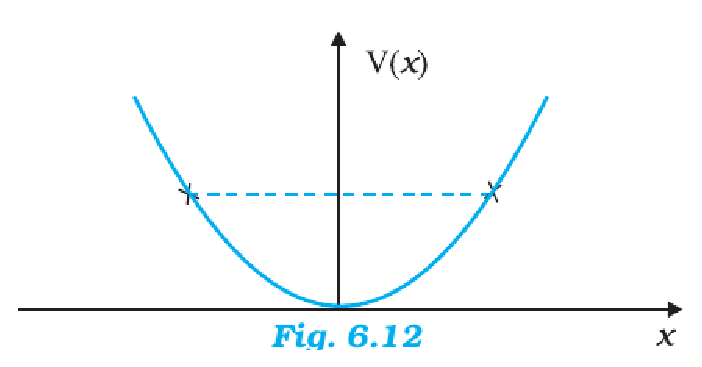
\includegraphics[width=\columnwidth]{./figs/11-1/6/6.12.eps}
\caption{}
\label{fig:6.10}
\end{figure}

\end{enumerate}
